\section{Finding and using LaTeX packages}
\label{sec:16}

\LaTeX\ not only delivers significant typesetting capabilities but also provides a framework for extensibility through the use of add-on packages. Rather than attempting to provide commands and features that “try to do everything”, \LaTeX\ is designed to be extensible, allowing users to load external bodies of code (packages) that provide more specialist typesetting capabilities or extend \LaTeX’s built-in features—such as typesetting tables. As observed in the section Adding images, the graphicx package extends \LaTeX\ by providing commands to import graphics files and was loaded (in the preamble) by writing

\begin{tcolorbox}
\begin{verbatim}
    \usepackage{graphicx}
\end{verbatim}
\end{tcolorbox}

\subsection{Loading packages}

As noted above, packages are loaded in the document preamble via the \verb|\usepackage| command but because (many) \LaTeX\ packages provide a set of options, which can be used to configure their behaviour, the \verb|\usepackage| command often looks like this:

\begin{tcolorbox}
\begin{verbatim}
    \usepackage[options]{somepackage}
\end{verbatim}
\end{tcolorbox}

The square brackets “\verb|[...]|” inform \LaTeX\ which set of options should be applied when it loads \verb|somepackage|. Within the set of options requested by the user, individual options, or settings, are typically separated by a comma; for example, the \href{https://ctan.org/pkg/geometry}{geometry package} provides many options to configure page layout in \LaTeX, so a typical use of geometry might look like this:

\begin{tcolorbox}
\begin{verbatim}
    \usepackage[total={6.5in,8.75in},
    top=1.2in, left=0.9in, includefoot]{geometry}
\end{verbatim}
\end{tcolorbox}

The \verb|geometry| package is one example of a package written and contributed by members of the global \LaTeX\ community and made available, for free, to anyone who wants to use it.

If a \LaTeX\ package does not provide any options, or the user wants to use the default values of a package’s options, it would be loaded like this:

\begin{tcolorbox}
\begin{verbatim}
    \usepackage{somepackage}
\end{verbatim}
\end{tcolorbox}

When you write \verb|\usepackage[...]{somepackage}| \LaTeX\ looks for a corresponding file called \emph{somepackage}.sty, which it needs to load and process—to make the package commands available and execute any other code provided by that package. If \LaTeX\ cannot find \emph{somepackage}.sty it will terminate with an error, as demonstrated in the following Overleaf example:

\begin{tcolorbox}
\begin{verbatim}
    \documentclass[12pt, letterpaper]{article}
    \usepackage{somepackage}% a NON-EXISTENT package
    \begin{document}
    This will fail!
    \end{document}
\end{verbatim}
\end{tcolorbox}

This example produces the following output:

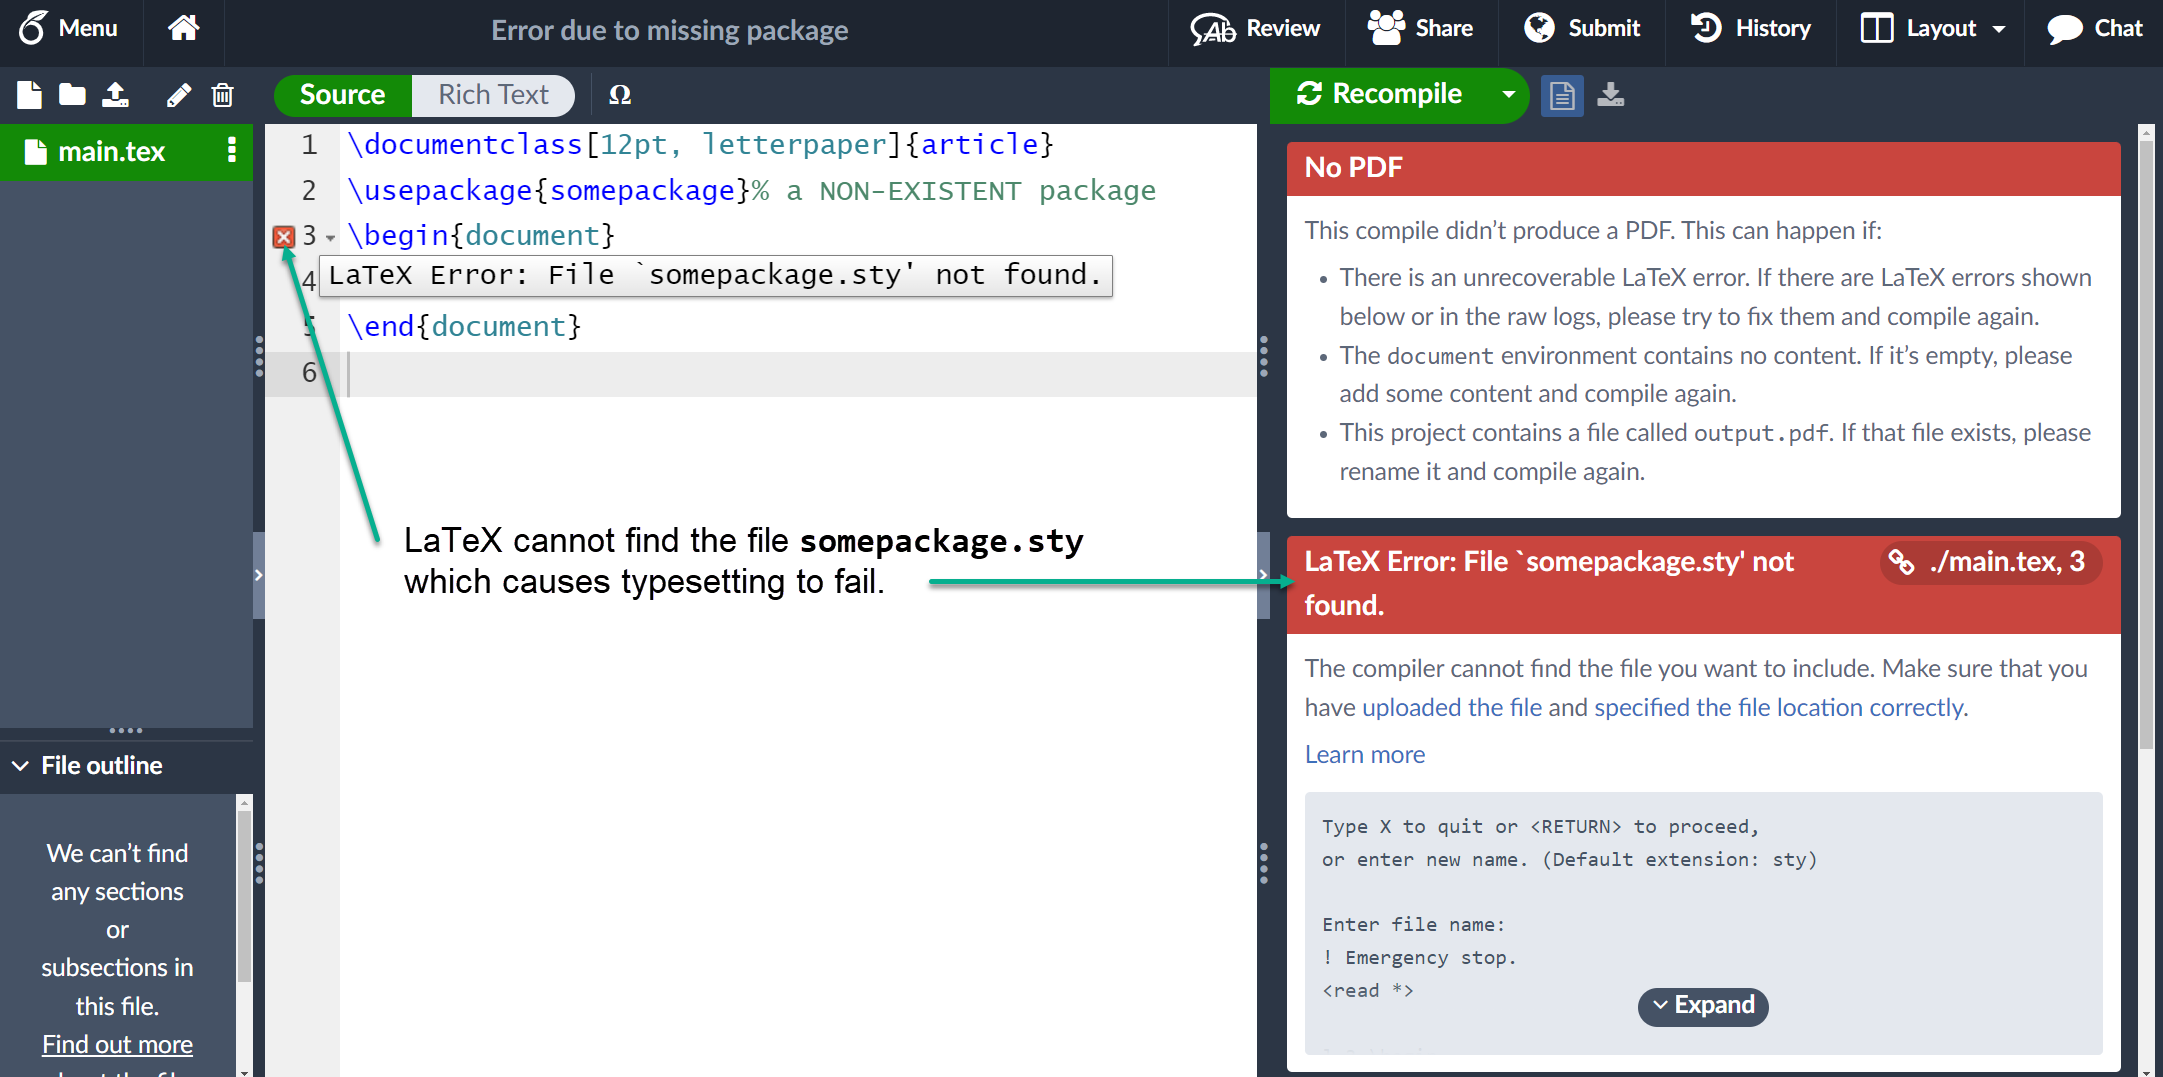
\includegraphics[width=\textwidth]{img16-1}

\subsection{Finding information about packages: CTAN}

Packages are distributed through the \href{https://www.ctan.org/}{Comprehensive TeX Archive Network}, usually referred to as CTAN, which, at the time of writing, hosts 6287 packages from 2881 contributors. CTAN \href{https://www.ctan.org/ctan}{describes itself} as

\quotebox{
... a set of Internet sites around the world that offer TEX-related material for download.
}

You can browse CTAN to look for useful packages; for example:

\begin{itemize}
    \item \href{https://www.ctan.org/topics/cloud}{by topic}
    \item \href{https://www.ctan.org/pkg}{alphabetically} (useful if you know the package name)
\end{itemize}

You can also use the \href{https://www.ctan.org/pkg}{search facility} (at the top of the page).

\subsection{Packages available on Overleaf: Introducing TeX Live}

Once per year a (large) \emph{subset} of packages hosted on CTAN, plus \LaTeX-related fonts and other software, is collated and distributed as a system called \href{https://tug.org/texlive/}{TeX Live}, which can be used to install your own (local) LaTeX setup. In fact, \href{https://www.overleaf.com/learn/latex/Overleaf_and_TeX_Live}{Overleaf’s servers also use TeX Live} and are updated when a new version of TeX Live is released. Overleaf’s TeX Live updates are not immediate but take place a few months post-release, giving us time to perform compatibility tests of the new TeX Live version with the \href{https://www.overleaf.com/gallery}{thousands of templates contained in our gallery}. For example, here is our \href{https://www.overleaf.com/blog/tex-live-2022-now-available}{TeX Live 2022 upgrade announcement}.

Although TeX Live contains a (large) \emph{subset} of CTAN packages it is possible to find an interesting package, such as \href{https://ctan.org/pkg/igo?lang=en}{igo for typesetting Go diagrams}, which is hosted on CTAN but not included in (distributed by) TeX Live and thus unavailable on Overleaf. Some packages hosted on CTAN are not part of TeX Live due to a variety of reasons: perhaps a package is obsolete, has licensing problems, is extremely new (recently uploaded) or has platform dependencies, such as working on Windows but not Linux.

New packages, and updates to existing ones, are uploaded to CTAN all year round but updates to TeX Live are distributed annually; consequently, packages contained in the current version of TeX Live will not be as up-to-date as those hosted on CTAN. Because Overleaf’s servers use TeX Live it is possible that packages installed on our servers—i.e., ones available to our users—might not be the very latest versions available on CTAN but, generally, this is unlikely to be problematic.